\chapter{Sistema}\label{solucion}

\begin{tcolorbox}[width=\textwidth,colback={white},title={\textbf{Lineamientos del Capítulo Sistema}},colbacktitle=black,coltitle=white]    
En este capítulo se deberá presentar de manera general la solución o arquitectura propuesta para resolver la problematica presenta. Para la descripción de la funcionalidad general y modular, se podrá apoyar de diagramas de bloques o conceptuales.
\end{tcolorbox}    


A continuación se presentan algunos ejemplos del uso de figuras, tablas, ecuaciones y referencias.


\section{Uso de Figuras}

Cada figura o diagrama que se incluya en el documento, debe ser correctamente referenciada y explicada, incluyendo la leyenda correspondiente \textbf{debajo de la figura}. Por ejemplo, en la Figura~\ref{fig:arch} se presenta la arquitectura general de una solución basada en IoT.

\begin{figure}[ht]
\centering
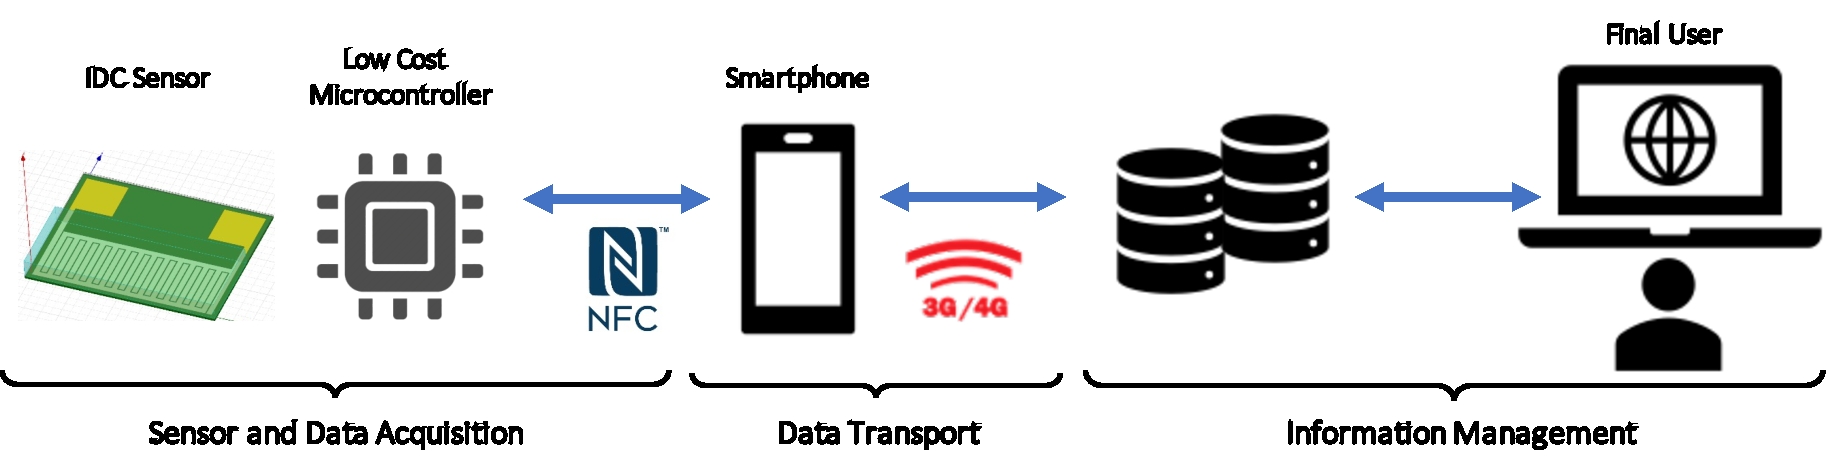
\includegraphics[width=15cm]{Cap3/arch.pdf}
\caption{Arquitectura de la solución basada en IoT.} \label{fig:arch}
\end{figure}

Se deberá privilegiar el uso de formatos vectoriales, por ejemplo pdf.


\section{Uso  de Tablas}

Cuando se requiera incluir tablas, cada columna deberá llevar un título y su correspondiente leyenda \textbf{encima de la tabla}. Como ejemplo se incluye la Tabla~\ref{tabla:capacitancia}.

\begin{table}[ht]
\begin{center}
\caption{Valor de la capacitancia utilizando sensores grandes y variando la capa aislante.}
\scalebox{1}[1]{
\begin{tabular}{| l | c | c | c|}
\hline
 \textbf{Parámetro} & \textbf{Sensor 1} & \textbf{Sensor 2} & \textbf{Sensor 3} \\
\hline
\hline
 Largo [cm] & 10.5 & 10.5 & 14 \\
%\hline
Ancho [cm] & 8 & 8 & 10.5 \\
%\hline
Aislante & Laca & Pintura & Laca \\
%\hline
Aire [nF] & $71.5\ensuremath{\times 10^{-3}}$ & 65.6 & 96.2 \\
%\hline
Agua destilada [nF] & $251\ensuremath{\times 10^{-3}}$ & 1.24 & 2.75 \\
%\hline
Concentración Tipo 1 [nF] & $358\ensuremath{\times 10^{-3}}$ & 1.8 & 140 \\
%\hline
Concentración Tipo 2 [nF] & $360\ensuremath{\times 10^{-3}}$ & 3 & 195 \\
%\hline
Concentración Tipo 3 [nF] & $380\ensuremath{\times 10^{-3}}$ &	3.2 & 228 \\
\hline
\end{tabular}}
\label{tabla:capacitancia}
\end{center}
\end{table}


\section{Uso de Ecuaciones}

Cuando se requiera, se podrán incluir ecuaciones siguiendo el ejemplo de la Ecuación~\ref{Eq1}:

\begin{equation} \label{Eq1}
k_1=\left(1+\frac{2a}{2d+b}\right) \sqrt{\frac{1+b/d}{(1+a/d+b/d)(1+a/d)}}
\end{equation}


\section{Uso de Referencias}

Cuando se deba incluir una referencia bibliográfica, se deberá incluir en el archivo \texttt{biblio.bib}, utilizando Bibtex y siguiendo el formato IEEEtrans~\cite{referencia1}.
